\section{The Conversational Structure of Problem-Solution Co-Evolution}
\label{sec:conversational-structure}

This section investigates on how control happens in \gls{oss}. Especially, we investigate on the how collaborative processes unfold when several users are free to join existing software projects as contributors. To gather insights on this process, we focus on the conversational aspect of the collaboration. To this end, we used speech act theory to analyze conversations between developers. We generated as dataset from manually encoded \glspl{pr} into speech acts \citep{searle1985expression}. Then, we analyzed these data through log analyses techniques and were able to pinpoint the nature of such conversational processes. The following sections describe the problem, approach and findings.

\subsection{Control Mechanisms in Software Development}

Open source software (OSS) development has become an important domain for studies who seek to explain the dynamics of new ways of organizing. In particular, \gls{floss} projects have been brought as an example of innovative ways of self-organizing \citep{DBLP:journals/mansci/KroghH06,DBLP:journals/misq/HowisonC14}. Works in literature have emphasized iterations (\citealp{Berente2005,Berente2007}), self-organization \citep{DBLP:journals/infsof/CrowstonLWEH07,DBLP:journals/jss/HodaM16} and free-speech \citep{DBLP:conf/chiir/ThomasCMCM18,Gibson2019}. 
%2. What is the overall problem or situation in that domain

Initiatives like the free software movement have often been understood as ``taking freedom" in participating to open source projects, studying its underlying ideas, changing the code, and redistributing the code to other users who are allowed the same freedom. In other words, open source software development has been seen as a libertarian practice (i.e., emphasizing individualism, freedom of choice and voluntary association) \citep{stallman2002free}. However, it has been shown that control mechanisms (be there social or institutional) are present in the area \citep{Lindberg2016}. In particular, online collaborative work that generates knowledge goes through "negotiation" actions which “pull” the trajectory and shape its movement in the feature space \citep{Arazy2020}. Therefore, it remains underexplored whether open source software development to what extent \gls{oss} is institutionalized and what are its similarities to corporate bureaucracy.


In the following, we addresses the problem of freedom in open source development by comparing it to corporate bureaucracy. We analyze pull requests from a real world open source repository using speech act theory. This, in combination with data analysis techniques and process mining, allows us to untangle interesting insights about OSS development and point out relevant resemblance to stage-gate processes. 

\Cref{fig:conversational-approach} gives an overview of the adopted approach for analyzing the processes that lie behind collaborative work. It follows a three-step process. First, we generate a structured dataset of the conversations from a number of software repositories. Second, we create an enriched event log which contains a mapping of each conversation to one or more speech acts. Third, we analyze the enriched event log to gather process insights on the conversation. Finally, we use these insights to better understand the domain. Next, we describe each of the steps. 

\begin{figure}
	\centering
	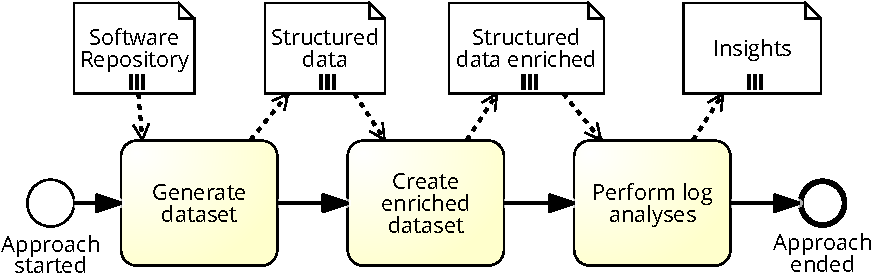
\includegraphics[width=0.8\linewidth]{figures/convesational-approach}
	\caption[Approach for analyzing conversations in software repositories]{Approach for analysing conversations in software repositories}
	\label{fig:conversational-approach}
\end{figure}



%\begin{inparadesc}
%	\item[Generate dataset.] dsadsada
%	
%	\item[Create enriched dataset.] 
%	
%	\item[Perform log analysis.] 
%	
%\end{inparadesc}

\subsubsection{Generating the dataset}

Our approach focuses on data from Github\footnote{https://github.com}, which stores more than 42 million public repositories\footnote{https://github.com/search?q=is:public}. A repository may contain several pieces of information related to software development such as a record of all the changes to the codebase, documentation and configuration files, and a forum that enables users to communicate with one another through message posting. 

In this context, collaboration happens as follows. When users want to contribute to an existing project, they first clone the repository into their local machine. After they have made the desired contribution (e.g., implemented a new feature) they need to make a request for integrating their contribution to the main codebase. Such request takes the name of \glsfirst{pr}. Pull requests have to undergo code-reviews in before the code is accepted and integrated to the code base. Such code-reviews are accompanied by conversations about the status of the work and may require several iterations before the code is ready to be merged or is the change is not accepted. Finally, the \gls{pr} can be closed. 

In order to generate a dataset from \glspl{pr} we proceed as follows. Aware of several perils \citep{DBLP:journals/ese/KalliamvakouGBS16} of using Github data, we selected a repository that is active and has been widely studied in other works \citep{Zhang2016,Lindberg2016,DBLP:conf/wcre/ConstantinouM17}. We wrote a script that extracts the first 600 pages of the Ruby on Rails (rails/rails) repository\footnote{https://github.com/rails/rails} as of March 2019. 
In order to have information about the complete lifecycle of conversations, we only extracted \glspl{pr} that were closed. This resulted in a dataset that comprised \glspl{pr} between August 2012 and February 2019. 

As a result we could organize the dataset in a tabular format that contains the following columns. \emph{Pull request number} is a unique identifier for each \gls{pr}. \emph{First user} is the person who opened the \gls{pr}. \emph{Status} indicates the decision taken on the \gls{pr} (i.e., merged or not merged). \emph{Timestamps} provide temporal information about when a \gls{pr} was opened and closed. \emph{Text} reports the comment from users. \emph{User} is the person who posted the comment. \emph{Timestamp} is the time in which the comment was posted. 


\subsubsection{Creating the enriched dataset}

This phase takes as input the structured dataset created previously and generates a new dataset in which each comment is mapped to a set of speech acts. 
We adopted the taxonomy provided by \cite{DBLP:journals/cscw/RipocheS06}. This taxonomy adapts the original work of \cite{searle1985expression} to the computer science domain. We further adapted their taxonomy to the Github conversations. In particular, we use the categories described in \Cref{tab:speech-act-types}. 

% Please add the following required packages to your document preamble:
% \usepackage{booktabs}
% \usepackage{multirow}
% \usepackage{graphicx}
\begin{table}[]
\centering
\caption{Speech acts used for analyzing pull requests}
\label{tab:speech-act-types}
\resizebox{!}{!}{%
\begin{tabular}{@{}ll@{}}
\toprule
Main Category                & Sub-Categories            \\ \midrule
Assertives                   & statement/description     \\ \hdashline
\multirow{2}{*}{Commissives} & commit                    \\
                             & offer                     \\ \hdashline
\multirow{5}{*}{Directives}  & request                   \\
                             & prescription/requirement  \\
                             & question                  \\
                             & instruction/suggestion    \\
                             & summon                    \\ \hdashline
\multirow{7}{*}{Expressives} & opinion/expression        \\
                             & acknowledgement/agreement \\
                             & disagreement              \\
                             & exclamation/emoji         \\
                             & apology                   \\
                             & greeting                  \\
                             & thank                     \\ \hdashline
Performatives                & action                    \\ \hdashline
\multirow{3}{*}{Others}      & code                      \\
                             & welcome comment           \\
                             & citation                  \\ \bottomrule
\end{tabular}%
}
\end{table}

We have further adapted the taxonomy to accommodate the discourse elements found in pull requests by grouping existing sub-categories and adding new elements. First, we have grouped together the categories \emph{statement} and \emph{description} as there is no substantial difference when it comes to pull requests. Then, we also grouped together  \emph{prescription} and \emph{requirement}, \emph{instruction} and \emph{suggestion}, \emph{opinion} and \emph{expression},  \emph{acknowledgments} and \emph{agreement}, and \emph{exclamation} and \emph{exmoji}. By combining these classes, we easy the task of categorizing comments. This is especially important when it comes to building an automatic classifier. 

We also included an additional category \emph{Others} to express three further speech acts we able to find in \glspl{pr}, respectively \emph{code}, \emph{welcome comment} (or simply \emph{welcome}) and \emph{citation}. Code indicates a fragment of code in the \gls{pr}. Welcome comment, indicates an automatic text generated by a bot in the moment a pull request is open. Citation indicates any part in which there is a reference to a previous comment. In the latter case, the citation may also quote an existing comment. The quoted message is treated as a duplicate in the annotation phase. 

To annotate the various posts we proceed as follows. We scan all the sentences of the post and find all the speech acts. Thus, each post is annotated with multiple speech act categories. First, we check whether a message falls into category \emph{Other}. This category is exclusive (i.e., the message is not further labeled with other speech acts). For example, all messages generated by a bot are classified into the welcome category and no other categories are allowed. All the rest, is classified into one of the remaining categories. Each sentence can have multiple speech acts. However, a word is only categorized into one specific speech act. An exception are the categories \emph{summon} and \emph{emoji} as they can express multiple speech acts. \Cref{tab:annotation-rules} summarizes the annotation rules.

% Please add the following required packages to your document preamble:
% \usepackage{booktabs}
% \usepackage{graphicx}
% \usepackage[table,xcdraw]{xcolor}
% If you use beamer only pass "xcolor=table" option, i.e. \documentclass[xcolor=table]{beamer}
\begin{table}[]
	\centering
	\caption{Speech acts annotation rules}
	\label{tab:annotation-rules}
	\resizebox{!}{!}{%
		\begin{tabular}{@{}lm{5.5cm}p{3cm}@{}}
			\toprule
			\multicolumn{1}{c}{\textbf{Speech Act Category}} &
			\multicolumn{1}{c}{\textbf{Instruction}} &
			\multicolumn{1}{c}{\textbf{Example}} \\ \midrule
			\begin{tabular}[c]{@{}l@{}}Statement\\ Description\end{tabular} &
			\textit{Something general, describing how something is (but not a procedure, this would be an instruction) referring to a different source closing a Pull Request,} &
			This PR fixes bug \#213213 \\
			\rowcolor[HTML]{EFEFEF} 
			Commit &
			\textit{Expresses a commitment of a user to doing something.  A promise is also a commitment.} &
			I will, Let me try \\
			Offer &
			\textit{We a user offers something to another user (e.g., to do a task for him)} &
			I can do, Happy to \\
			\rowcolor[HTML]{EFEFEF} 
			Request &
			\textit{When a user asks another user to do something.} &
			Do task A,  Can you please fix this \\
			\begin{tabular}[c]{@{}l@{}}Requirement\\ Prescription\end{tabular} &
			\textit{It describes how something should be, what is needed or what has to be done in order to fulfill a need, necessity or criteria} &
			I need, This should be, must/needs to \\
			\rowcolor[HTML]{EFEFEF} 
			Question &
			\textit{When a users poses a question} &
			What do you think? Can I? How? \\
			\begin{tabular}[c]{@{}l@{}}Suggestion\\ Instruction\end{tabular} &
			\textit{Parts of texts that contain instructions about how to do something} &
			Maybe you can try, I would suggest, First do A \\
			\rowcolor[HTML]{EFEFEF} 
			Summon &
			\textit{When a user tags another user with @} &
			@rails-bot \\
			\begin{tabular}[c]{@{}l@{}}Opinion\\ Expression\end{tabular} &
			\textit{When somebody expresses an opinion.} &
			I think, As far as I am concerned, I believe \\
			\rowcolor[HTML]{EFEFEF} 
			\begin{tabular}[c]{@{}l@{}} {\cellcolor[HTML]{EFEFEF}Acknowledgment}\\ Agreement\end{tabular} &
			\textit{When a user expresses positive feelings about a comment from another user} &
			I like your idea, OK, Sounds good, Good job \\ 
			Disagreement &
			\textit{When a user expresses disagreement} &
			No, I don’t think so, I am against \\
			\rowcolor[HTML]{EFEFEF} 
			\begin{tabular}[c]{@{}l@{}}\cellcolor[HTML]{EFEFEF}Emoji\\ Exclamation\end{tabular} &
			\textit{When the comment contains and emoji, smiley or phrases expressing exclamation} &
			:), \textless{}3 \\
			Apology &
			\textit{When a user apologizes for something} &
			Sorry, My bad, forgive me \\
			\rowcolor[HTML]{EFEFEF} 
			Greeting &
			\textit{Includes different types of greetings} &
			Hi, Hello, Welcome \\
			Thank &
			\textit{When a user thanks someone} &
			Thanks, Thank you \\
			\rowcolor[HTML]{EFEFEF} 
			Action &
			\textit{When a part of the phrase means that the user did something. This only applies when the users talk in first person. If the users says that someone else did something, then it is not an action but rather a statement.} &
			I did, We fixed, Done, I solved \\
			Code &
			\textit{A listing that represents code. They are enclosed in ```} &
			```ruby\_x005F\_x000D\_``` \\
			\rowcolor[HTML]{EFEFEF} 
			Citation &
			\textit{Citations include any quotation to existing message or its parts. In the extracted data the are always preceded by the symbol \textless{}} &
			\textgreater So, I want an isolated plug-n-play \\ \bottomrule
		\end{tabular}%
	}
\end{table}

\subsubsection{Performing log analysis and gathering insights}

After the dataset is annotated with speech acts, the next step is to apply analyses tools in order to gather insights. 
In order to do so, we exploit process mining tools like Disco and ProM. These tools enable us to perform several types of analyses, including basic statistics, trace and model-based. The input of these techniques is an event log in the \gls{xes} format. 

The outcome of this step is a set of insights about the conversational process. Especially, we are interested in the analyses that may unveil corporate bureaucracy aspects in \gls{oss}. In particular, we look into 
\begin{inparaenum}[\itshape i)]
	\item how the different speech acts are distributed and what are the characteristics of the different types of pull requests
	\item whether there are pattern of users who represent central decision makers, and
	\item what speech acts are associated to the different users.
\end{inparaenum}



\subsection{Results}

In the following we describe the results of this approach on the Ruby on Rails repository. 

\subsubsection{Speech acts distribution and pull request process}

The manually annotated 2072 \glspl{pr} from the Ruby on Rails\footnote{https://github.com/rails/rails} repository have the following distribution of speech acts. Statements and descriptions are by far the most common types of speech. This is also in line with findings from previous studies \citep{DBLP:journals/cscw/RipocheS06,DBLP:conf/sigsoft/WoodRAM18} about conversations in this domain. 

\begin{figure}
	\centering
	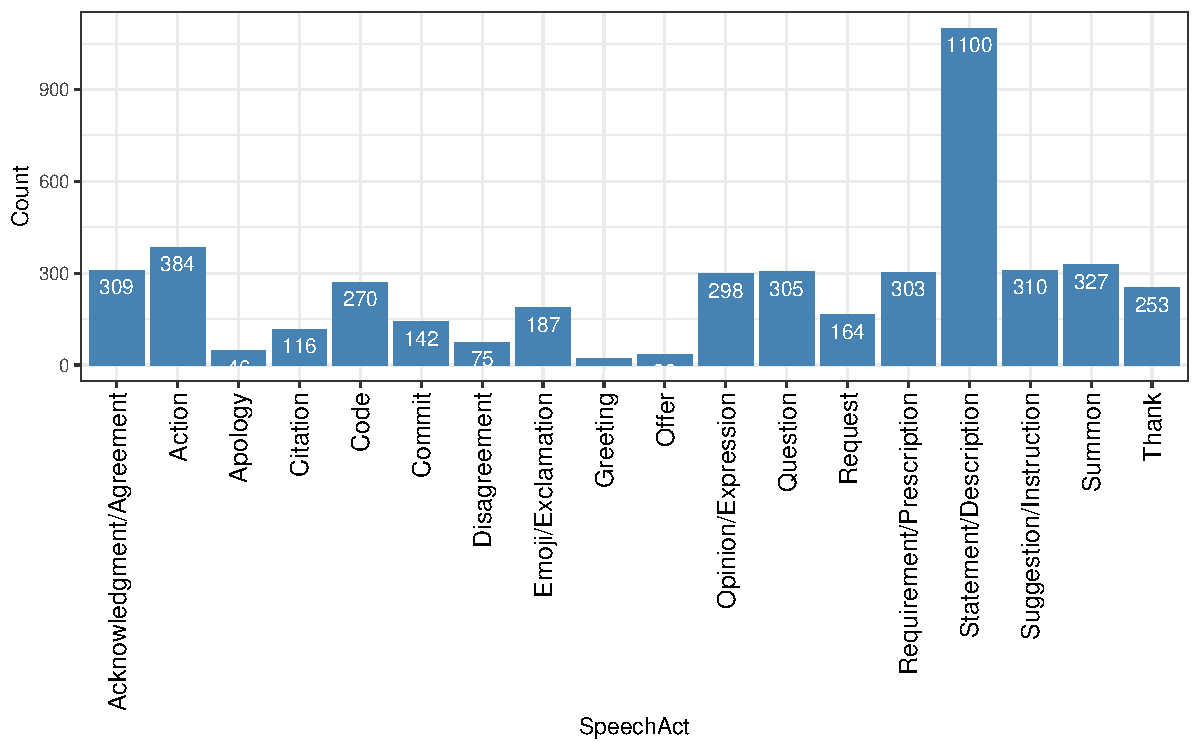
\includegraphics[width=\linewidth]{figures/speechActCount}
	\caption[Speech act categories manually annotated on Rails project]{Distribution of the speech act categories in the manually annotated conversations of the Rails project}
	\label{fig:speechactcount}
\end{figure}


Other frequent categories are acknowledgment, action, code, opinion, question, requirement, suggestion, summon or thank. These categories were found in ten to twenty percent of the posts. There are also quite evenly distributed, suggesting that these categories are represent the types of speech which are actually used, while statement seems like a ``must-have'' speech act. The remaining categories occurred below ten percent and they may be considered as unusual speech acts. The category ``welcome'' is not reported in the plot as it only occurred three times. 


% TODO: Continue here

Reducing the distinct number of activities for process mining was performed
as follows. First, the categories citation, emoji, summon, greeting and were
excluded as they were not considered relevant for process mining. As the
category welcome per definition excludes other Speech Act annotations and
can not occur in combined annotations, this category was not adapted.
The remaining categories were combined iteratively to create a smaller set
of annotations. Similar categories should be merged, showing the occurrence
of either or both of the original categories. Then, these categories should be
combined to activities, by listing and separating them with a comma. This
should result in data sets for manual and automatic annotation, showing
simplified annotations that can then be used for process mining.
The simplified annotation framework consists of the categories, that can
be seen in Table 10. The categories of statement and action were consid-ered similar enough to be merged. Whereas statement includes Speech Acts
defining how something is, action defines a new state that was reached by
doing an action. In addition to that, the distinction between statement and
action of who did something was neglected for process mining. Question and
request contain either asking something or asking someone to do something.
As they contain similar phrases and distinction between them is less clear
than for other categories, they are merged for process mining. Commit and
offer both contain information about someone potentially doing something in
future which also includes similar phrases. Therefore, these categories were
also merged.
Suggestion, opinion and requirement all include more or less subjective
Speech Acts on how something should be or should be done. To a certain de-
gree, the categories share the structure of suggesting future action or desired
outcomes of future action, which was a reason to merge them. As disagree-
ment was not found to be similar with other categories, only its name was

simplified to Di. All of the above described simple categories should always
be included in the combined activity used for process mining, if they occurred
in a certain comment.
The categories thank and acknowledgement were merged, as they share
similar characteristics, both expressing agreement or positive feelings towards
others, their actions or their work. In contrast to the other simplified cate-
gories, ThaAck is considered less relevant and will therefore only be included
in the activity, if there is no other annotation available for a certain com-
ment. In addition to that, code will only show as the activity, if it is the only
annotation available for a comment.
The described simplification of categories resulted in 30 distinct activities
in the manually annotated data set and 36 activities in the automatically
annotated comments.
To further explore if patterns of Speech Acts appear in cycles, the distinct
activities that were created during simplification of annotations, were con-
secutively numbered based on their appearance in the Pull Request. As the
highest number of occurrences of certain categories is found to be 16, adding
the number to the categories would again result in a very large amount of
distinct activities. Therefore, only the numbers 2, 3 and 3+, for more than 3
occurrences, were added to the activity. This was done with a Visual Basic
script in Excel. Within each comment, it consecutively numbers equal com-
binations of Speech Acts in a new column. Then, only 2, 3 and 3+ are joined
with the annotations accordingly.

% Please add the following required packages to your document preamble:
% \usepackage{booktabs}
% \usepackage{graphicx}
\begin{table}[h]
	\centering
	\caption{Aggregation of similar speech acts onto macro-categories}
	\label{tab:aggregated-categories}
	\resizebox{!}{!}{%
		\begin{tabular}{@{}cc@{}}
			\toprule
			\textbf{Aggregated Category} & \textbf{Consituting Categories}  \\ \midrule
			StaAct                       & statement, action                \\
			QueReq                       & question, request                \\
			ComOff                       & commit, offer                    \\
			SugOpiRequi                  & suggestion, opinion, requirement \\
			Dis                          & disagreement                     \\
			ThaAck                       & thank, acknowledgement           \\
			Code                         & code                             \\ \bottomrule
		\end{tabular}%
	}
\end{table}

\Cref{tab:aggregated-categories} shows the aggregation of similar categories. 

\begin{figure*}[h]
	\centering
	\begin{subfigure}[b]{\linewidth}
		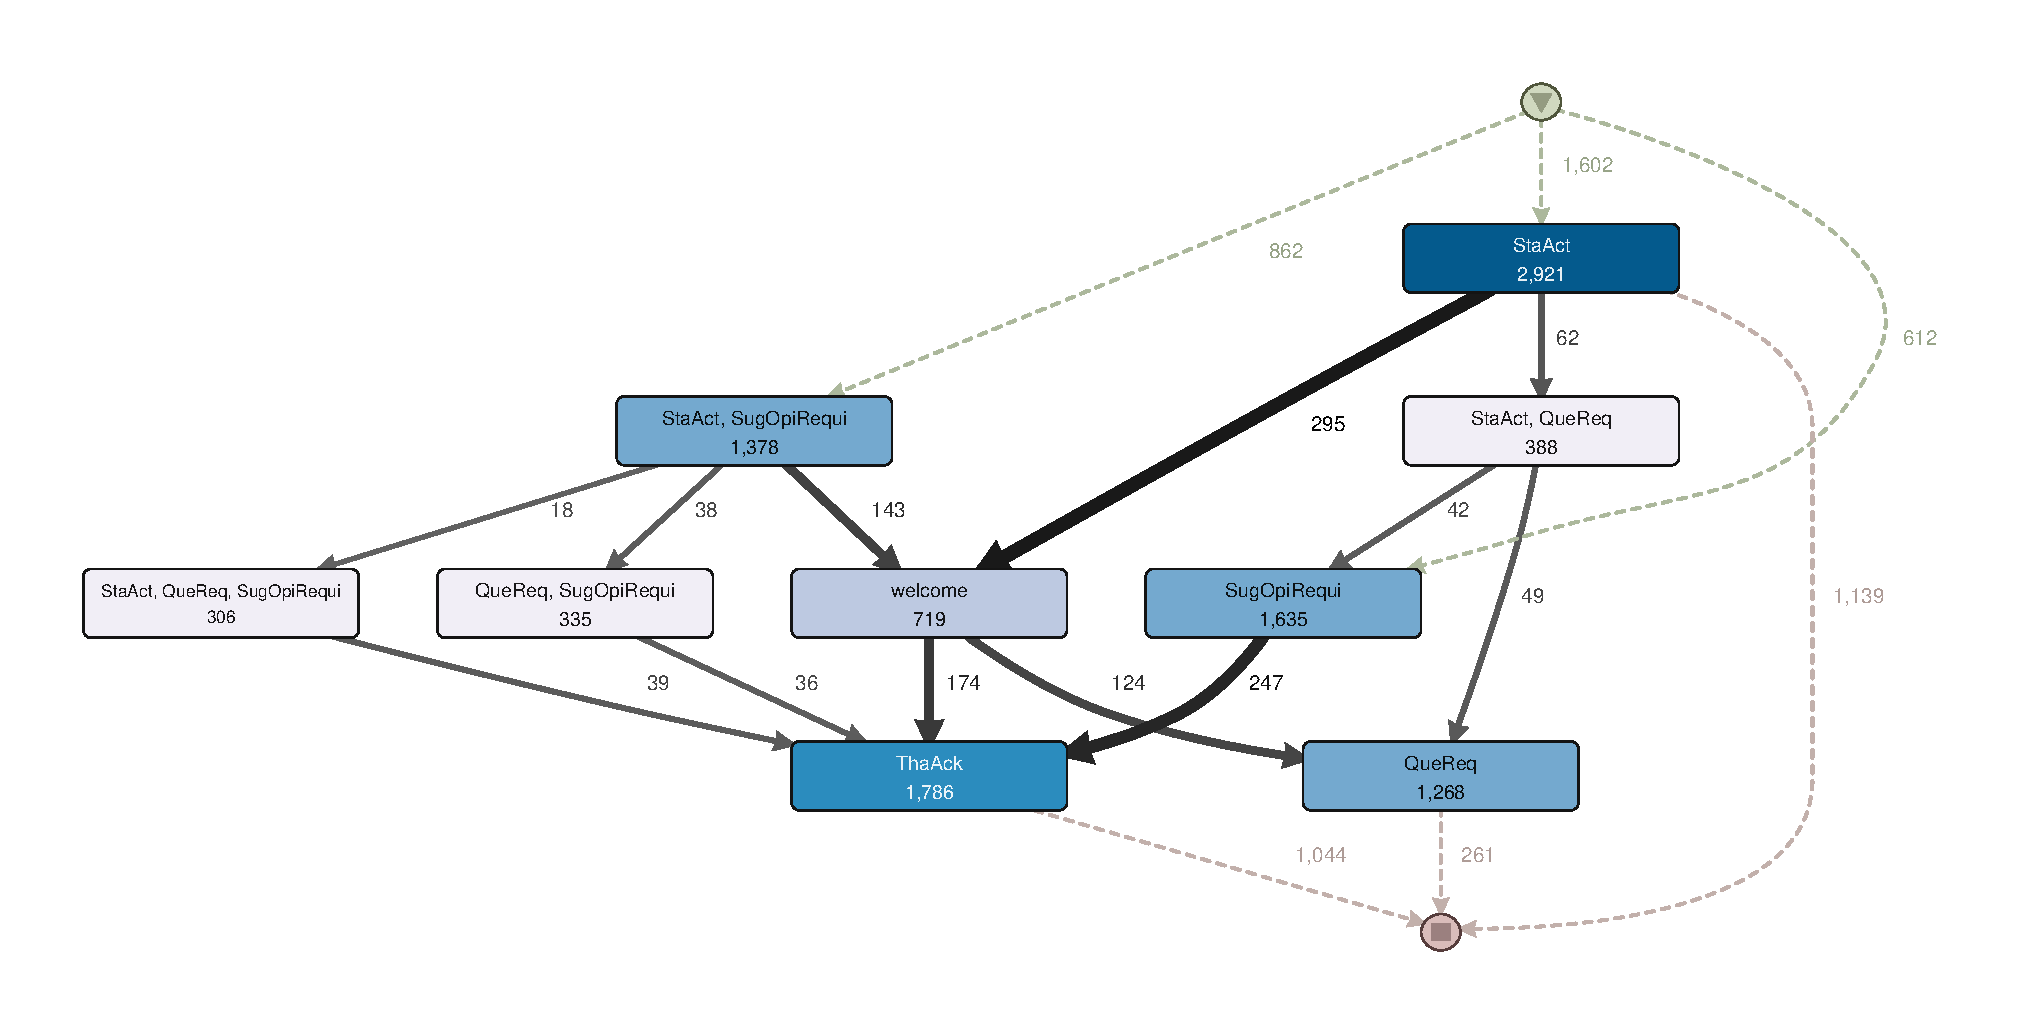
\includegraphics[width=.98\linewidth]{figures/merged-a25-p0}
		\caption{Merged pull requests}
	\end{subfigure}
%
	\begin{subfigure}[b]{\linewidth}
		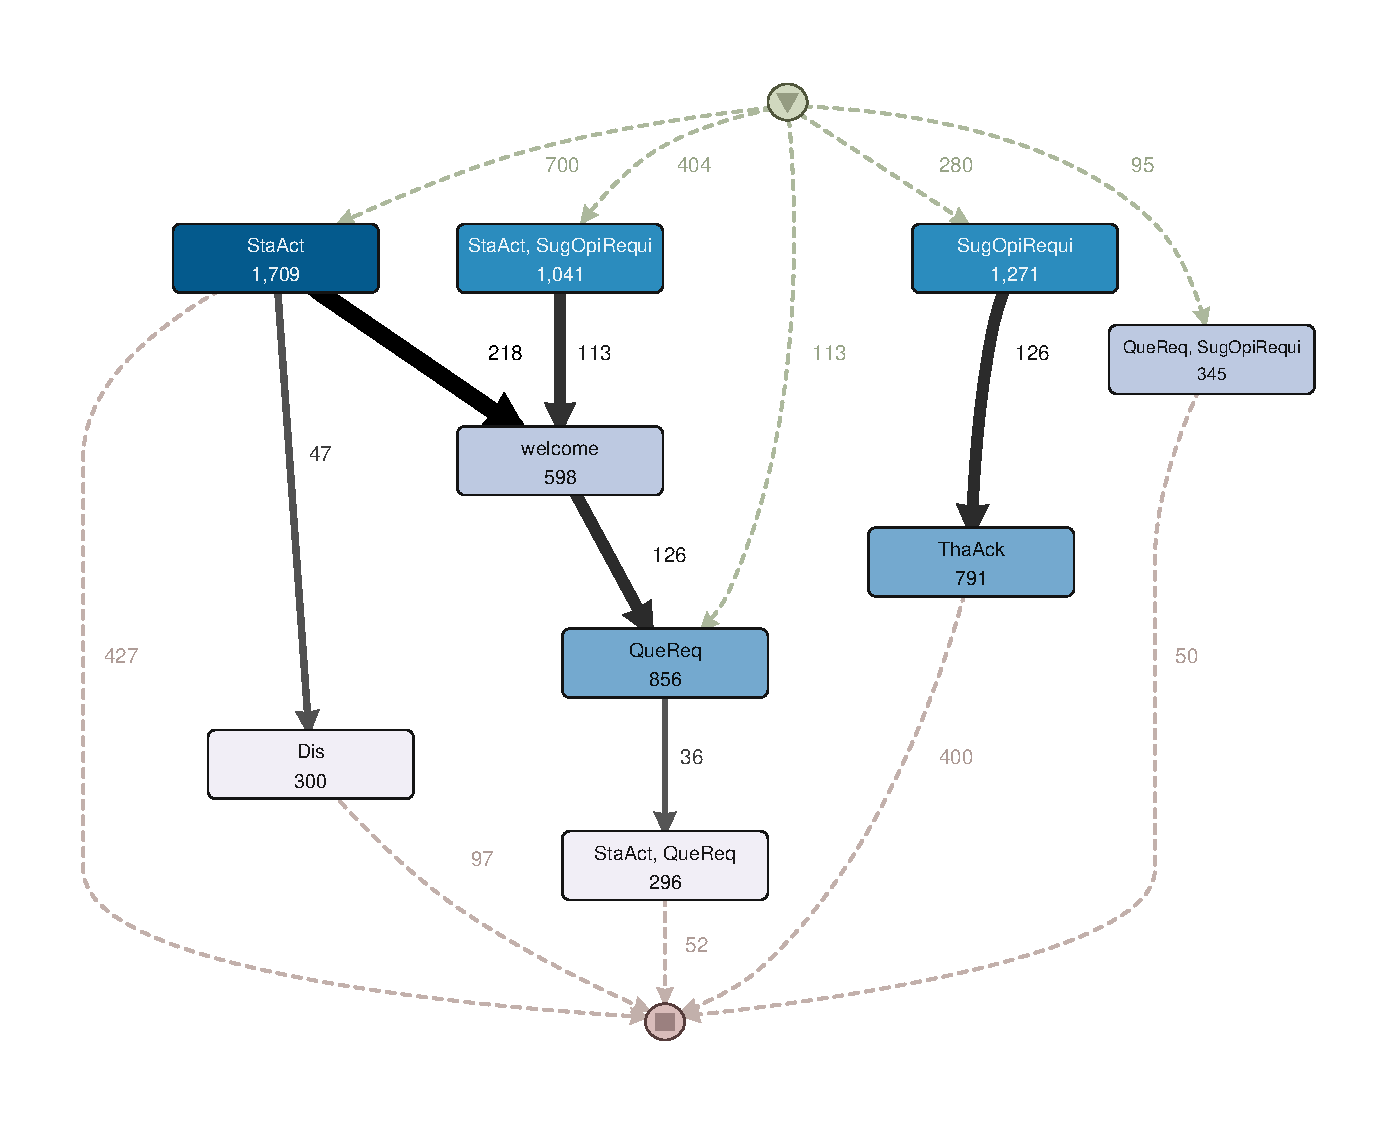
\includegraphics[width=.98\linewidth]{figures/not-merged-a25-p0}
		\caption{Not merged pull requests}
	\end{subfigure}
	\label{fig:speechActProcess}
\end{figure*}

\subsubsection{Gate keepers in OSS}

We use graphstream\footnote{https://graphstream-project.org/} a java library for representing and working with dynamic graphs \citep{DBLP:journals/corr/abs-0803-2093}. 

\begin{figure}[h]
	\centering
	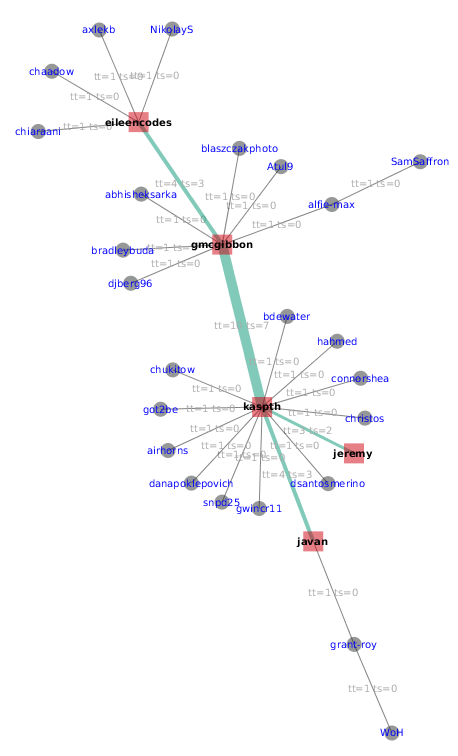
\includegraphics[width=0.7\linewidth]{figures/socio-graph}
	\caption[Subgraph of all the interactions in a group]{Subgraph of all the interactions that happened within a connected component in a social network}
	\label{fig:socio-graph}
\end{figure}

\Cref{fig:socio-graph} shows this graph 

\subsubsection{User specialization}

\begin{figure}[h]
	\centering
	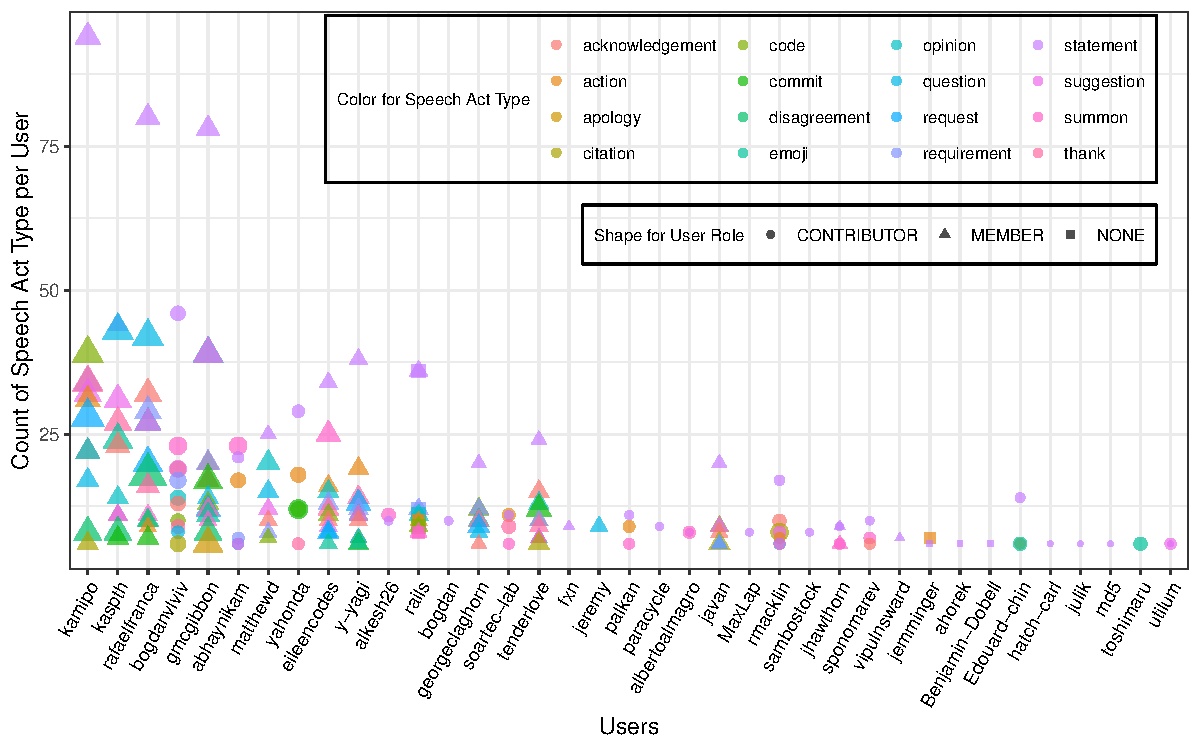
\includegraphics[width=\linewidth]{figures/speechActTypesPerUser}
	\caption{Speech act categories per user type}
	\label{fig:speech-act-types-per-user}
\end{figure}

\Cref{fig:speech-act-types-per-user} shows the different kinds of user



Whereas many Pull Requests finish after a few number of comments, others were found to take multiple years. On Rails/Rails repository on GitHub, the number of comments per Pull Request can range up to 155, considering all closed Pull Requests \cite{noauthor_pull_railsrails_nodate}. By analyzing a random selection of 6 short and 6 long Pull Requests, the following qualitative differences were found. Whereas in short Pull Requests, the described problem could be solved fast, long Pull Requests include more discussion on how to approach the task. However, this could also mean that it was clear very fast, that a certain problem needed more work. This could then result in a Pull Request being closed after a few comments, with the remark that the issue would be addressed in another Pull Request. This leads to the assumption that in short Pull Requests, the problem is defined more clearly and a decision whether to merge or not to merge can be reached faster, even if the decision is that the task should be performed in another way. 

Consisting of 20 to 30 comments, longer Pull Requests were found to contain discussions between at least two users. An aspect resulting in more comments was found to be the initiating user repeatedly offering to adapt and improve their code. This could also include asking how to perform changes to fulfill the requirements and have their Pull Request merged. 

Based on the work of Tötzl \cite{thesisgithub}, the speech acts found in the initial comments usually included statements, whereas later comments included more subjective speech acts like opinions and suggestions. The final comments were then found to contain thank and acknowledgments towards the participating users and their work. Despite the higher number of comments, there were few repetitions of the phases found. % means that once users started suggesting, they would not go back to posting only statements

Another finding of longer Pull Requests was that if the initial comment did not include a final solution but contained suggestions on how to approach some issue, more comments usually followed, where users started discussing their ideas. In addition to that, Pull Requests could also be rejected after long discussions on whether the proposed feature was required and should be added. 


